\section{Visuelles System}
Das visuelle System dient zur Verarbeitung visueller Information und umfasst Auge, Sehnerv und Teile des Gehirns.

\subsection{Das Auge}
Das Auge ähnelt in seiner Funktion einer Kamera. Die Linse (das Objektiv) sammelt Lichtstrahlen und projiziert diese als auf dem Kopf stehendes gespiegeltes Bild auf die Netzhaut (den Film). Da der Abstand zwischen Linse und Netzhaut (die Bildweite) unveränderlich ist, muss die Brechkraft (Brennweite) der Augenlinse angepasst werden. Diese Anpassung nennt man \textit{Akkommodation}.
% TODO: Besseres Bild?
\begin{figure}
	\centering
	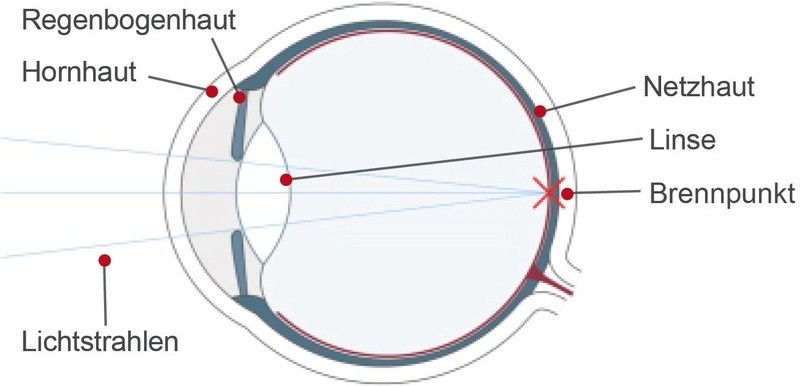
\includegraphics[width=7cm]{images/auge.jpg}
	\caption{Das Auge \cite{auge}}
\end{figure}

Das lichtempfindliche Organ sind die Sehzellen der Netzhaut.